% Tento soubor nahraďte vlastním souborem s přílohami (nadpisy níže jsou pouze pro příklad)

% Pro kompilaci po částech (viz projekt.tex), nutno odkomentovat a upravit
%\documentclass[../projekt.tex]{subfiles}
%\begin{document}

% Umístění obsahu paměťového média do příloh je vhodné konzultovat s vedoucím
%\chapter{Obsah přiloženého paměťového média}

%\chapter{Manuál}

%\chapter{Konfigurační soubor}

%\chapter{RelaxNG Schéma konfiguračního souboru}

%\chapter{Plakát}

\chapter{Pokyny pro sestavení programu}

Tato příloha obsahuje podrobné pokyny pro vytvoření spustitelného souboru ze zdrojového kódu. Program je přeložitelný na operačních systémech \emph{Windows} a~\emph{Linux}. Překlad byl testován konkrétně na systémech \emph{Windows 11} a~Linuxové distribuci \emph{Ubuntu, verze 22.04}. Program by také mělo být možné přeložit na operačním systému \emph{macOS}, nicméně zde testování překladu neproběhlo.

\section*{Sestavení na operačním systému Windows}

Na operačním systému \emph{Windows} doporučuji používat systém \emph{MSYS2}\footnote{\url{https://www.msys2.org/}}. Tento systém umožňuje jednoduchou správu nástrojů a~knihoven pomocí prostředí připomínající \emph{Arch Linux}. Z~oficiálních stránek \emph{MSYS2} si stáhněte instalační program a~systém si nainstalujte. Ihned po instalaci doporučuji provést aktualizaci systému \emph{MSYS2}: otevřete aplikaci \emph{MSYS2~MINGW64} a~zadejte tento příkaz:
\begin{verbatim}
    pacman -Syu
\end{verbatim}
Pomocí nástroje \texttt{pacman} určeného pro správu balíčků se provede aktualizace všech balíčků. Poté z~aplikace \emph{MSYS2~MINGW64} nainstalujte tyto balíčky:
\begin{itemize}
    \item překladač \emph{GCC}/\emph{G++},
    \item nástroj \emph{Git},
    \item nástroj \emph{Make},
    \item nástroj \emph{CMake},
    \item knihovny \emph{SDL2}, \emph{SDL2\_image} a~\emph{SDL2\_ttf},
    \item knihovnu \emph{CGAL}.
\end{itemize}
K~tomu použijete tyto příkazy:
\begin{verbatim}
    pacman -S mingw-w64-x86_64-gcc
    pacman -S git
    pacman -S make
    pacman -S mingw-w64-x86_64-cmake
    pacman -S mingw-w64-x86_64-SDL2
    pacman -S mingw-w64-x86_64-SDL2_image
    pacman -S mingw-w64-x86_64-SDL2_ttf
    pacman -S mingw-w64-x86_64-cgal
\end{verbatim}

Adresář \texttt{source/} přesuňte z~paměťového média do některého z~adresářů prostředí\linebreak \emph{MSYS2} (například do \verb|/home/<vaše-jméno>/|) a~v~aplikaci \emph{MSYS2~MINGW64} přejděte příkazem \texttt{cd} do adresáře \texttt{source/}. Zde zadejte tento příkaz:
\begin{verbatim}
    git submodule update
\end{verbatim}
Z~\emph{GitHubu} se stáhnou knihovny \emph{libSDL2pp}, \emph{yaml-cpp} a~\emph{ImGui}. Nyní by mělo být vše připraveno k~sestavení. Přejděte do adresáře \texttt{source/src/} a~zadejte tyto 2~příkazy:
\begin{verbatim}
    cmake .
    cmake --build . --config Release
\end{verbatim}
Poté, co se tyto příkazy úspěšně dokončí, bude v~adresáři \texttt{source/} vygenerován soubor \texttt{BUBLRAWL.exe}, který můžete nyní spustit.

\section*{Sestavení na operačním systému Linux}

Sestavení na operačním systému \emph{Linux} probíhá obdobným způsobem jako na operačním systému \emph{Windows}. Tentokrát však není třeba instalovat žádný pomocný systém. Pomocí správce balíčků vaší distribuce \emph{Linuxu} nainstalujte balíčky:
\begin{itemize}
    \item překladač \emph{GCC}/\emph{G++},
    \item nástroj \emph{Git},
    \item nástroj \emph{Make},
    \item nástroj \emph{CMake}\footnote{V~některých distribucích může mít správce balíčku verzi nástroje \emph{CMake}, která není nejnovější. Proto doporučuji jej stáhnout přímo z~oficiálních stránek a~nainstalovat manuálně podle přiloženého souboru \texttt{README}: \url{https://cmake.org/download}},
    \item knihovny \emph{SDL2}, \emph{SDL2\_image} a~\emph{SDL2\_ttf},
    \item knihovnu \emph{CGAL}.
\end{itemize}
Poté přejděte do adresáře \texttt{source/} a~stáhněte si další potřebné knihovny pomocí tohoto příkazu:
\begin{verbatim}
    git submodule update
\end{verbatim}

Pokud vše proběhlo úspěšně, mělo by být nyní možné program sestavit. Přejděte do adresáře \texttt{source/src/} a~zadejte tyto příkazy:
\begin{verbatim}
    cmake .
    cmake --build . --config Release
\end{verbatim}
Po úspěšném dokončení těchto příkazů se v~adresáři \texttt{source/} nacházet spustitelný soubor \texttt{BUBLRAWL}. Je ale také pravděpodobné, že tyto příkazy selžou. Většinou se problém týká knihoven, které \emph{CMake} nedokáže najít. Pokud je chyba hlášena v~knihovně \emph{libSDL2pp}, může pomoci úprava souboru \texttt{CMakeLists.txt} v~adresáři \texttt{source/libSDL2pp/}: pokud nástroj \emph{CMake} hlásí chybějící knihovnu \verb|SDL2_ttf::SDL2_ttf|, najděte v~souboru \texttt{CMakeLists.txt} řádek, kde se tato knihovna vyhledává, a~změňte název knihovny na \verb|SDL2_ttf| (odstraňte část za dvěma dvojtečkami včetně těchto dvojteček). Stejným způsobem lze v~tomto souboru vyřešit problém s~knihovnou \emph{SDL2} nebo \emph{SDL2\_image}. Pokud ani toto nepomůže, pak zkuste nainstalovat problematické knihovny manuálně. Pomocí správce balíčků odinstalujte problematickou knihovnu, poté stáhněte zdrojové soubory této knihovny z~oficiálního úložiště a~proveďte instalaci podle pokynů. Oficiální úložiště jednotlivých knihoven jsou následující:
\begin{itemize}
    \item \emph{SDL2}: \url{https://github.com/libsdl-org/SDL/releases}
    \item \emph{SDL2\_image}: \url{https://github.com/libsdl-org/SDL_image/releases}
    \item \emph{SDL2\_ttf}: \url{https://github.com/libsdl-org/SDL_ttf/releases}
    \item \emph{CGAL}: \url{https://github.com/CGAL/cgal/releases}
\end{itemize}



\chapter{Dotazník}
\label{app:dotaznik}

\newcommand{\questionnairemultipleoptions}[2]{
\noindent\begin{minipage}{\textwidth}
\textbf{#1}\\[1em]
\begin{tikzpicture}
    % Some tricks to force decimal comma.
    % https://tex.stackexchange.com/a/525641
    \pgfkeys{/pgf/number format/use comma}
    \pie[text=legend, before number=\pgfmathprintnumber, radius=2.5]{#2}
\end{tikzpicture}
\end{minipage}
\bigskip
}

\newcommand{\questionnairecheckboxes}[4]{
\noindent \begin{minipage}{\textwidth}
\textbf{#1}\\[1em]
\begin{tikzpicture}
    \begin{axis}[
        width=11.6cm,
        height=#2,
        %enlargelimits=0.2,
        xbar,
        xmin=0,
        symbolic y coords={#3},
        ytick=data,
        nodes near coords,
    ]
    \addplot coordinates {#4};
    \end{axis}
\end{tikzpicture}
\end{minipage}
\bigskip
}

\newcommand{\questionnairecheckboxesbots}[8]{\questionnairecheckboxes{#1}
{7cm}
{Ladybug, Blind predator, Blind prey, Wall-aware predator, Wall-aware prey, A* predator, Minimax prey}
{(#2,Ladybug) (#3,Blind predator) (#4,Blind prey) (#5,Wall-aware predator) (#6,Wall-aware prey) (#7,A* predator) (#8,Minimax prey)}
}

\newcommand{\questionnairetextanswer}[4]{
\noindent \begin{minipage}{\textwidth}
\textbf{#1}\\[1em]
\begin{tikzpicture}
    \begin{axis}[
        /pgf/number format/use comma,
        bar width=#2,
        width=\textwidth,
        height=0.25\textheight,
        enlargelimits=0.2,
        ybar,
        symbolic x coords={#3},
        xtick=data,
        point meta=y/11*100,
        nodes near coords={\pgfmathprintnumber[precision=1]{\pgfplotspointmeta} \%},
    ]
    \addplot coordinates {#4};
    \end{axis}
\end{tikzpicture}
\end{minipage}
\bigskip
}

\newcommand{\questionnairelinearrange}[8]{
\noindent \begin{minipage}{\textwidth}
\textbf{#1}\\[1em]
\begin{tikzpicture}
    \begin{axis}[
        /pgf/number format/use comma,
        bar width=1.5cm,
        width=\textwidth,
        height=0.25\textheight,
        enlargelimits=0.2,
        ybar,
        symbolic x coords={1,2,3,4,5},
        xtick=data,
        point meta=y/11*100,
        nodes near coords={\pgfmathprintnumber[precision=1]{\pgfplotspointmeta} \%},
        xlabel={\makebox[14cm]{\small #7 \hfill #8}}, % An odd approach, innit?
    ]
    \addplot coordinates {(1,#2) (2,#3) (3,#4) (4,#5) (5,#6)};
    \end{axis}
\end{tikzpicture}
\end{minipage}
\bigskip
}

\newcommand{\questionnairefreetext}[2]{
\noindent \begin{minipage}{\textwidth}
\textbf{#1}
#2
\end{minipage}
\bigskip
}

\newcommand{\questionnairefreetextanswer}[1]{\begin{quote}
    #1
\end{quote}}

V~této příloze se nachází otázky z~dotazníku o~aplikaci \emph{Bubble Brawl}, a~také souhrnné statistiky odpovědí. Dotazník vyplnilo celkem 11 uživatelů, kteří si vyzkoušeli základní funkce, které aplikace nabízí. Otázky byly rozděleny do několika sekcí podle toho, kterého prvku aplikace se týkají. Pro vytvoření dotazníku byla použita aplikace \emph{Google Forms}\footnote{\url{https://www.google.com/forms/about/}}, která následně poskytla také souhrn odpovědí.

\section*{Vzhled a navigace}

\questionnairelinearrange{Byla navigace (hlavní menu, spuštění hry, ukončení hry, …) dostatečně intuitivní? Bylo jednoduché přijít na to, co které tlačítko dělá a~kam Vás zavede?}
{4}{5}{1}{1}{0}
{velmi intuitivní}{málo intuitivní}

\questionnairelinearrange{Byla navigace pohodlná?}
{2}{7}{2}{0}{0}
{velmi pohodlná}{málo pohodlná}

\questionnairelinearrange{Jak na Vás působila aplikace vzhledově?}
{2}{5}{3}{1}{0}
{hezká}{ošklivá}

\section*{Hraní hry}

\questionnairelinearrange{Bavilo Vás hru hrát?}
{5}{5}{1}{0}{0}
{velmi bavilo}{vůbec nebavilo}

\questionnairetextanswer{Kolik her jste odehráli (do konce, nebo alespoň dostatečně dlouho)?}
{1.4cm}
{2,3,5,6,7,10}
{(2,1) (3,1) (5,3) (6,1) (7,1) (10,4)}

\questionnairemultipleoptions{Přibližně kolik času jste celkově věnovali hraní hry?}
{9.1/Méně než 5 minut, 9.1/5--10 minut, 45.5/10--20 minut, 36.3/Více než 20 minut}

\questionnairelinearrange{Bylo jednoduché přijít na to, jak se hra hraje a~co je cílem?}
{4}{4}{3}{0}{0}
{velmi jednoduché}{velmi obtížné}

\questionnairelinearrange{Jak hodnotíte ovladatelnost?}
{9}{1}{0}{1}{0}
{dobrá ovladatelnost}{špatná ovladatelnost}

\questionnairelinearrange{Jak dobře byla hra vybalancovaná? Nebylo příliš jednoduché dostat se do vedení, nebo naopak příliš obtížné vyřadit ostatní hráče?}
{2}{5}{1}{1}{2}
{dobře vybalancovaná}{špatně vybalancovaná}

\questionnairelinearrange{Byla hra dostatečně rozmanitá? Nebo Vám po chvíli začala připadat příliš repetitivní?}
{3}{2}{5}{1}{0}
{velmi rozmanitá}{málo rozmanitá}

\questionnairemultipleoptions{Běžela hra dostatečně rychle nebo bylo poznat, že se „seká“? Zaměřte se prosím pouze na hry, kdy jste nepoužili umělou inteligenci.
}{100/Hra běžela dobře, 0/Hra se sekala}

\questionnairefreetext{Co dalšího byste o~hře chtěli říct (např. co byste přidali, co byste změnili, další názory na hru, …)? (volitelné)}{
    \questionnairefreetextanswer{Byla fajn}
    \questionnairefreetextanswer{Vzhled hry by šel vylepšit použitím antialiasingu u~fontů.\\
    Po dokončení hry bych uvítal okolo nápisu "Winner"{} nějaký zvýrazňující box do kterého se přesune tlačítko Quit.}
    \questionnairefreetextanswer{Chyběl mi nějaký tutorial, který by mě seznámil s~tím, co je cílem hry. Ukončení hry po výhře je umístěno zvláštně, čekal bych ho u~textu Winner nebo bych čekal automatické ukončení hry. Hra mě nijak neupozornila na to, že musím mít vybranou mapu, abych mohl přidat boty.}
    \questionnairefreetextanswer{Přidal bych možnost nějakých speciálních vlastností, aby se dala hra skutečně ukončit, protože v~jeden moment kdy je jeden hráč "malý"{} a~druhý "velký", tak se nemají šanci porazit}
    \questionnairefreetextanswer{Pri tvoreni vlastni hry chvili trvalo prijit na to, ze se objekty (walls) potvrzuji stisknutim praveho tlacitka mysi.}
}

\section*{Umělá inteligence ve hře}

\questionnairecheckboxesbots{Proti kterým typům „botů“ jste si zahráli?}
{9}{8}{8}{6}{7}{10}{7}

\questionnairecheckboxesbots{Který „bot“ byl podle Vás nejschopnější? Můžete vybrat i~více.}
{3}{0}{2}{1}{2}{6}{0}

\questionnairecheckboxesbots{Který „bot“ byl podle Vás nejslabší? Můžete vybrat i~více.}
{4}{1}{4}{0}{0}{1}{2}

\questionnairecheckboxesbots{Proti kterému z „botů“ bylo nejzábavnější hrát? Můžete vybrat i~více.}{3}{2}{3}{0}{0}{6}{3}

\questionnairemultipleoptions{Byla pro Vás hra zábavnější, když jste do hry zapojili „boty“ nebo byla hra lepší bez nich?}
{54.5/Byla zábavnější s~nimi, 9.1/Byla zábavnější bez nich, 36.4/Zážitek s~nimi i~bez nich byl srovnatelný}

\questionnairelinearrange{Jak dobře připomínali „boti“ chováním skutečné hráče?}
{0}{4}{3}{4}{0}
{velmi přesvědčivě}{málo přesvědčivě}

\questionnairetextanswer{Kolik nejvíce „botů“ jste do hry zapojili najednou?}
{1.4cm}
{1,2,3,4,6}
{(1,3) (2,3) (3,1) (4,2) (6,2)}

\questionnairemultipleoptions{Byl zřetelný pokles výkonu při zapojení „botů“ do hry?}
{0/{Ano, vždy}, 0/{Ano, ale pouze u~některých/pouze s~určitým počtem}, 100/Ne}

\section*{Editor mapy}

\questionnairetextanswer{Kolik map jste si v~editoru vytvořili nebo upravili?}
{1.6cm}
{0,1,2,3}
{(0,1) (1,3) (2,6) (3,1)}

\questionnairelinearrange{Bylo používání editoru dostatečně intuitivní? Dokázali jste přijít na to, jak dosáhnout toho, čeho jste chtěli a~jak fungují jednotlivá tlačítka a~nástroje?}
{2}{3}{4}{2}{0}
{velmi intuitivní}{málo intuitivní}

\questionnairelinearrange{Byla práce s~editorem pohodlná?}
{4}{5}{2}{0}{0}
{velmi pohodlná}{málo pohodlná}

\questionnairemultipleoptions{Zaznamenali jste při používání editoru pokles výkonu? V~jakých situacích?}
{0/Vždy, 0/Při velkém přiblížení, 0/Při velkém množství objektů, 100/Nikdy, 0/Jiné}

\questionnairefreetext{Chyběly Vám v~editoru nějaké funkce? (volitelné)}{
    \questionnairefreetextanswer{Nějaké tooltipy, čeho čím docílím}
    \questionnairefreetextanswer{ne}
}

\questionnairefreetext{Je něco dalšího, co byste o~editoru chtěli říct? (volitelné)}{
    \questionnairefreetextanswer{Někde bokem bych velmi stručně popsal základní ovládání, například není vůbec zřejmé, že lze v~editoru přibližovat. Dále při tvorbě zdí alespoň říci, že zeď se dokončí pravým kliknutím.}
    \questionnairefreetextanswer{Možná nějaký popis toho, co jaké čudlíky dělají.}
    \questionnairefreetextanswer{Není moc intuitivní a~chvíli mi trvalo, než jsem přišel na to jak se ovládá, ale jakmile jsem ho pochopil, tak bylo jeho používání snadné}
    \questionnairefreetextanswer{Pri tvoreni vlastni hry chvili trvalo prijit na to, ze se objekty (walls) potvrzuji stisknutim praveho tlacitka mysi.}
}

\section*{Závěr}

\questionnairefreetext{Našli jste při používání aplikace nějaké chyby (vizuální, funkcionální)? Pokud ano, napište, jak k~chybě došlo, a~pokud možno, zkuste popsat, jak chybový stav reprodukovat. Případně můžete také poslat snímek/záznam obrazovky na můj email. (volitelné)}{
    \questionnairefreetextanswer{Ne}
    \questionnairefreetextanswer{Nejsem si jistý zdali tomu tak je naschvál, ale při záměrné prohře proti botovi se objevil nápis "Winner". Očekával bych v~takové situaci, kdy hraji single-player spíše "Loser".}
}

\questionnairefreetext{Mohli byste prosím uvést informace o~Vašem počítači, na kterém jste hru hráli? (procesor, grafická karta, velikost RAM, operační systém) (volitelné)}{
    \questionnairefreetextanswer{Intel i5-4460, NVIDIA GTX 1060 6GB, 16GB DDR3, Win10}
    \questionnairefreetextanswer{Intel i5 13600K, Intel UHD Graphics 770, 32 GB DDR5 5600 MHz, Win 10}
    \questionnairefreetextanswer{Procesor - Intel Pentium Gold 7505\\
    Grafická karta - Intel UHD Graphics 630\\
    RAM - 8GB\\
    operační systém - Windows 11}
    \questionnairefreetextanswer{OS Win 10\\
    RAM 1X16 GB\\
    AMD Ryzen 5 2600 6 jader\\
    NVIDIA GeForce GTX 1660 OC}
    \questionnairefreetextanswer{Intel Core i5 (Broadwell-U), Intel HD Graphics 5500, 8GB, Windows}
}

\questionnairefreetext{Je něco dalšího co byste o~aplikaci chtěli říct? (volitelné)}{
    \questionnairefreetextanswer{Super}
    \questionnairefreetextanswer{Super hra}
    \questionnairefreetextanswer{moc povedené}
}


% \chapter{Diagram tříd}

% Tato příloha obsahuje diagram tříd, který reprezentuje strukturu programu. Jelikož je struktura programu velmi rozsáhlá, bylo nutné rozdělit diagram na několik částí.

% První část obsahuje proces příchodu události (například stisku klávesy) z~knihovny \emph{SDL} a~její následnou cestu ke kořenovému \emph{Controlleru}. Nachází se zde také třída \emph{Main}, která představuje hlavní tělo programu.

% Ve druhé části je znázorněn proces propagace události od kořenového \emph{Controlleru} k~jeho \uv{dítěti}. Je zde znázorněno, jak bylo implementováno odebírání a~zahazování událostí v~jednotlivých nekořenových \emph{Controllerech}.

% Ve třetí části je popsána třída, jež představuje rozhraní komunikaci s~\emph{SDL}; obecně s~čímkoliv, co poskytuje přístup k~uživatelskému vstupu a~výstupu.

% Diagram byl vytvořen pomocí nástroje \emph{draw.io}\footnote{\url{https://app.diagrams.net/}}.

% 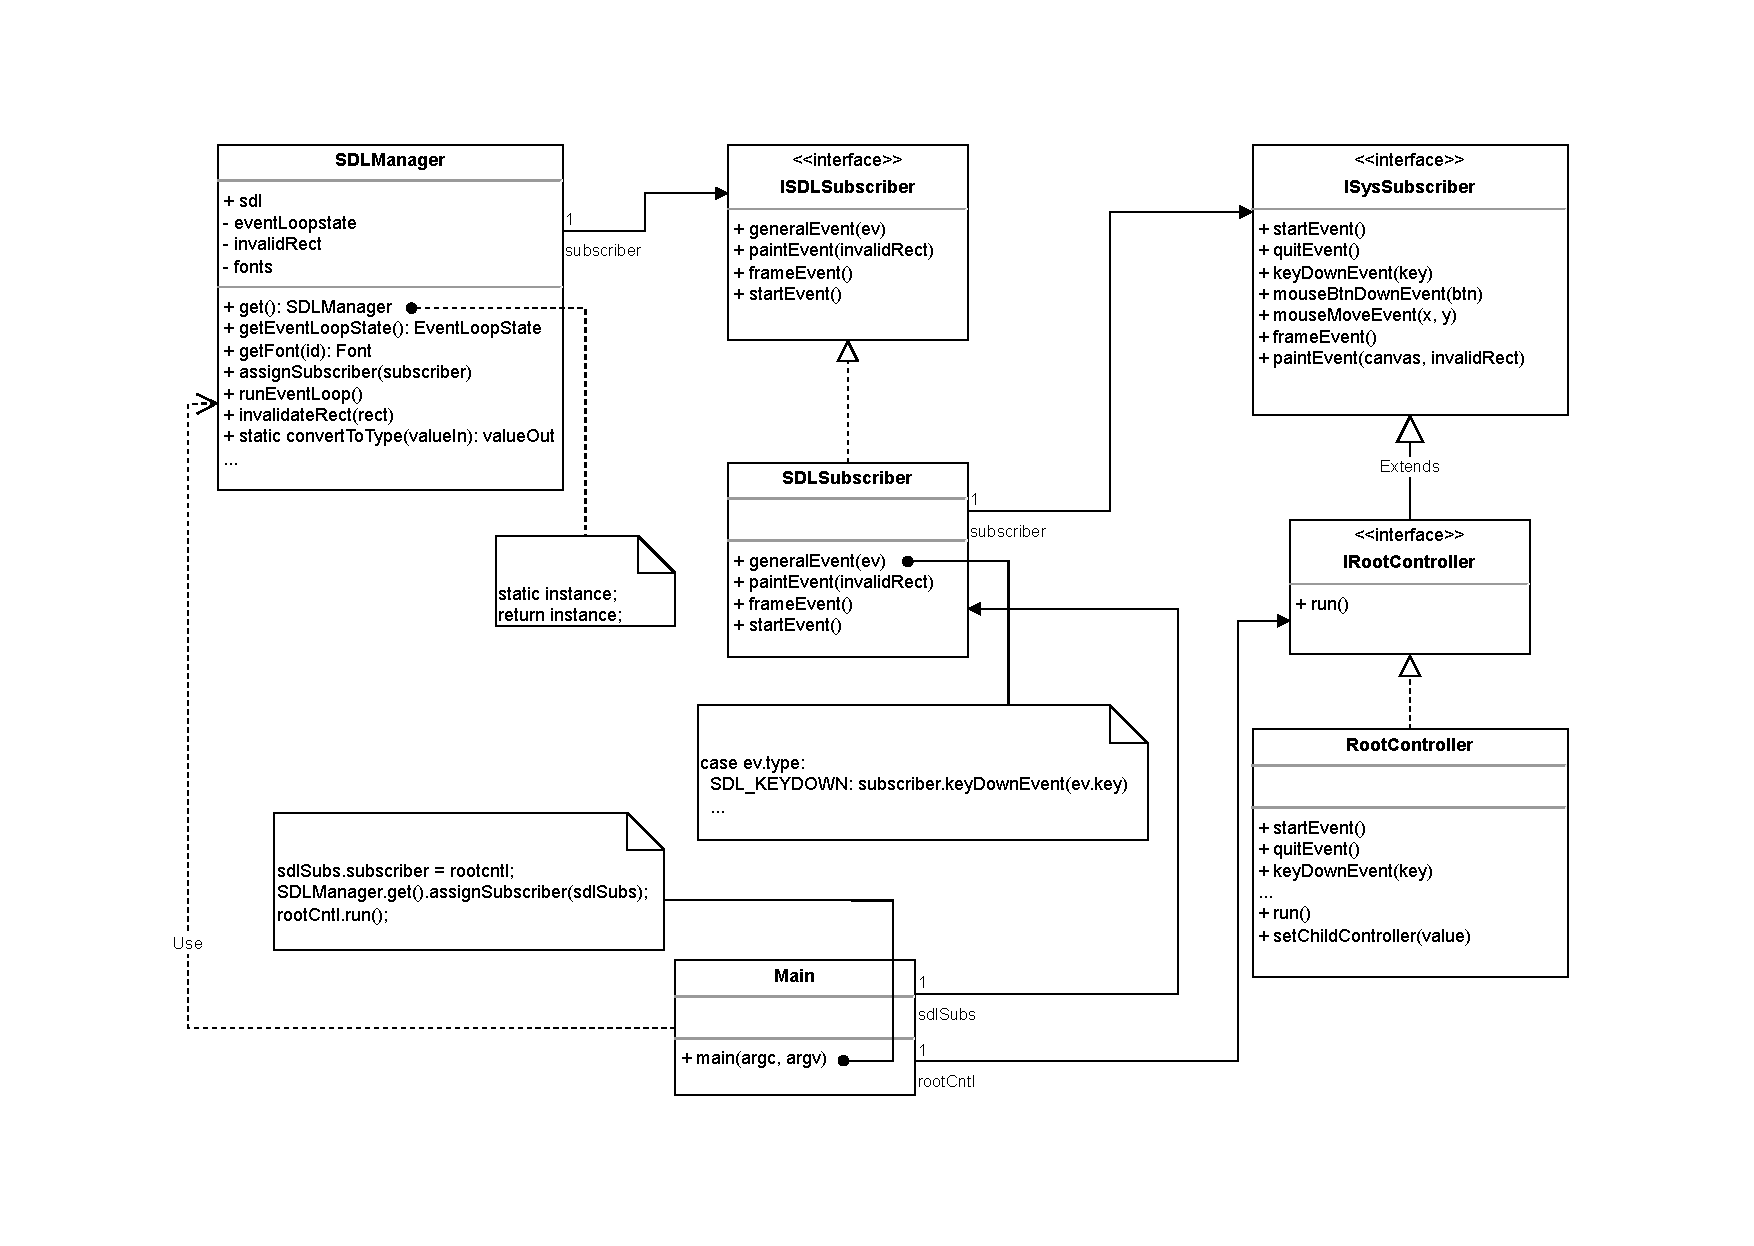
\includepdf[pages=-]{class-diagram.pdf}


% \chapter{Důkaz nekonečnosti stavového prostoru hry Bubble Brawl}
% \label{app:dukaz-nekonecnosti}

% Tato příloha dokazuje, že existuje nekonečně mnoho stavů, jakých může hra \emph{Bubble Brawl} nabývat. Důkaz se vztahuje k~jednomu hráči na herní ploše, jejíž rozměry jsou celá kladná (konečná) čísla, přičemž hráč \emph{nemění svoji velikost}. Výchozí stav hry je následující:
% \begin{itemize}
%     \item Na souřadnicích $[-50, -50]$ se nachází stěna překážky. Tato stěna pokračuje kolmo směrem dolů.
%     \item Na souřadnicích $[51 + \sqrt{2}, -50]$ se nachází jiná stěna překážky, která taktéž pokračuje kolmo směrem dolů.
%     \item Na souřadnicích $[0, 0]$ se nachází hráč, který má množství života stejné, jako na začátku hry.
%     \item Mezi těmito dvěma stěnami se nenachází žádní další hráči ani bonusy.
%     \item Šířka herní plochy je dostatečně velká, aby se do ní vlezly tyto 2 překážky. Výška herní plochy je dostatečně velká, aby se do ní vlezl hráč a~pod sebou měl alespoň $(1 + \sqrt{2}) + \frac{17}{6}$ místa.
% \end{itemize}
% Pro jednoduchost se uvažuje soustava souřadnic, jejíž souřadnice X roste směrem vpravo, souřadnice Y směrem dolů a~počátek soustavy je v~bodě, kde se nachází hráč. Stav hry je zobrazen na obrázku~\ref{fig:wa-bfs-predator-infinite}.

% \begin{figure}[ht]
%     \centering
%     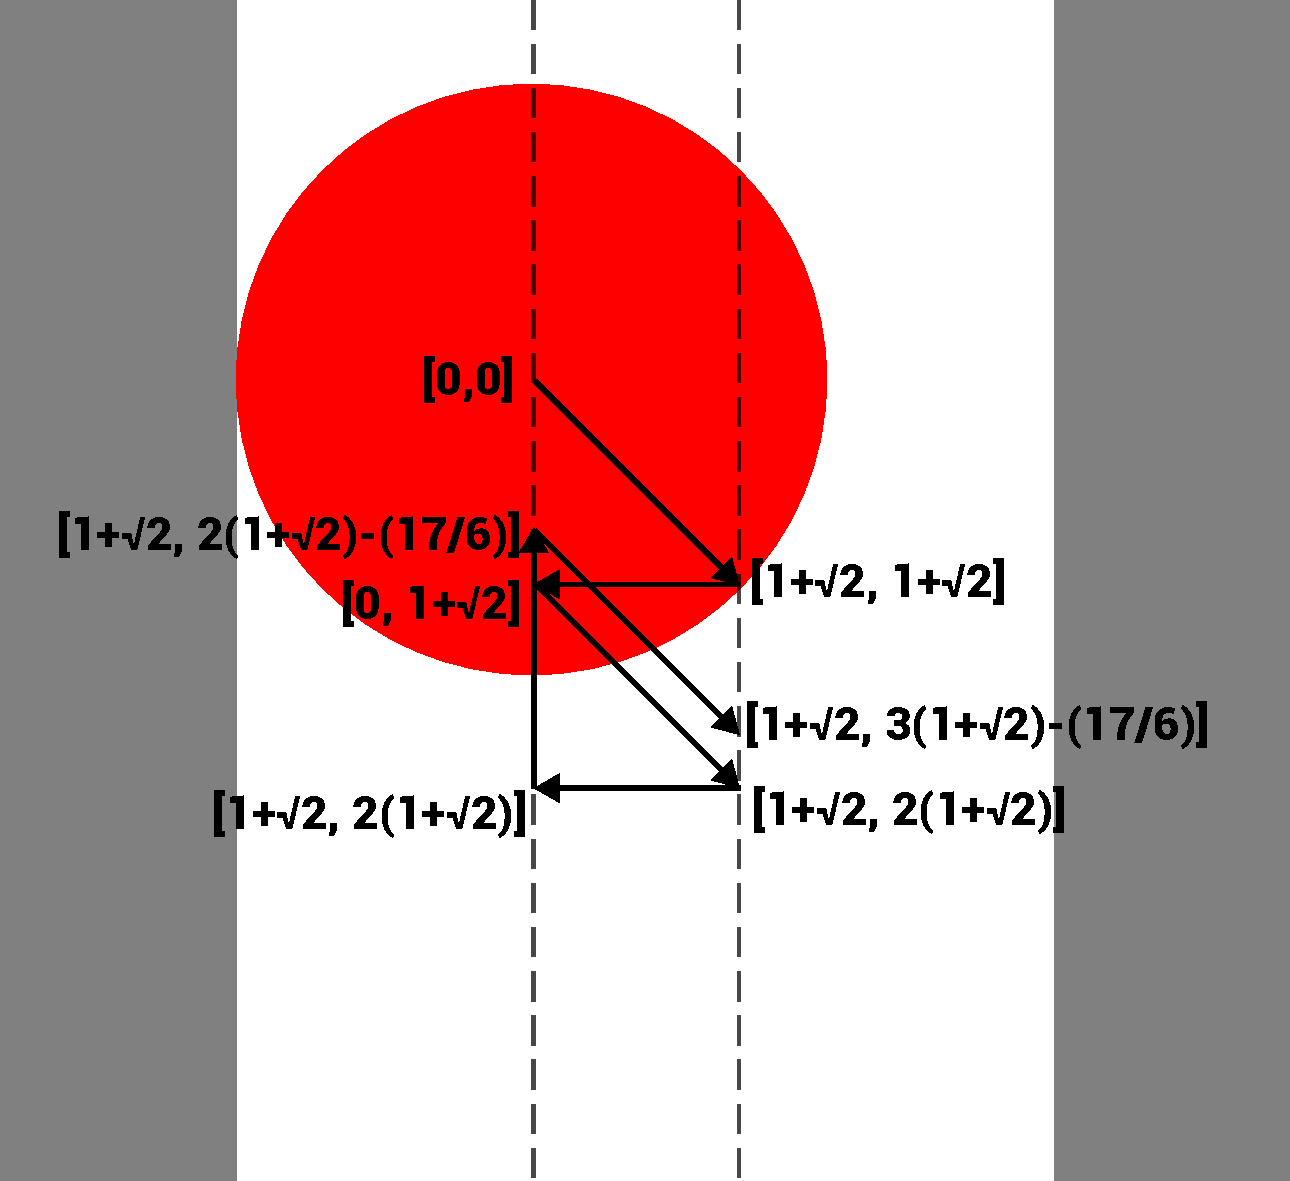
\includegraphics[width=0.8\textwidth]{doc/obrazky-figures/wa-bfs-predator-infinite.pdf}
%     \caption{Stav hry použitý pro důkaz. Černé šipky znázorňují pohyb hráče.}
%     \label{fig:wa-bfs-predator-infinite}
% \end{figure}

% Aby byl stavový prostor nekonečný, musí existovat nekonečná posloupnost kroků bez opakujících se stavů. Důkaz bude proveden sporem.

% Mějme tedy posloupnost stavů $(a_n)_{n = 1}^\infty$ generovanou tímto předpisem:
% \begin{equation}
%     (a_n)_{n = 1}^\infty,\quad a_n = \left\{\begin{array}{ll}
%         [0, 0] & \text{pro} n = 1 \\
%         a_{n-1} - (1 + \sqrt{2}, 0) & 
%     \end{array}\right.
% \end{equation}
% \begin{itemize}
%     \item pokud souřadnice X hráče není 0, a~tedy se dotýká pravé stěny, provede se pohyb vlevo. Jinak,
%     \item pokud je souřadnice Y hráče menší než $\frac{17}{6}$, provede se diagonální pohyb dolů doprava. Pozice hráče se tímto změní o~$(1 + \sqrt{2}, 1 + \sqrt{2})$. Jinak,
%     \item provede se pohyb nahoru. Pozice hráče se tímto změní o~$(0, \frac{17}{6})$.
% \end{itemize}
% Tato posloupnost je zobrazena na obrázku~\ref{fig:wa-bfs-predator-infinite}. Nyní předpokládejme, že tato posloupnost nekonečná \emph{není}. V~tom případě v~této posloupnosti existují 2~shodné stavy.


% \chapter{Algoritmus pro výpočet trajektorií hráčů}
% \label{app:vypocet-trajektorii-hracu}

% V~této příloze je popsán nepoužitý algoritmus pro výpočet trajektorií pohybu hráčů. Tento algoritmus nebyl použit, protože se nepovedlo přijít s~implementací, která by byla dostatečně výkonná. Nicméně je zde uveden pro případ, kdyby se povedlo výkon algoritmu optimalizovat.

% Algoritmus se snaží na herní ploše simulovat působení sil na entity hráčů. Stisk klávesy simuluje sílu působící na entitu požadovaným směrem. Při kolizi s~překážkou na entitu působí síla kolmá k~povrchu překážky. Tím pádem při nárazu do překážky entita dále pokračuje v~pohybu podél překážky, avšak s~menší rychlostí, a~pohyb tak působí přirozeně.

% \begin{figure}[ht]
%     \centering
%     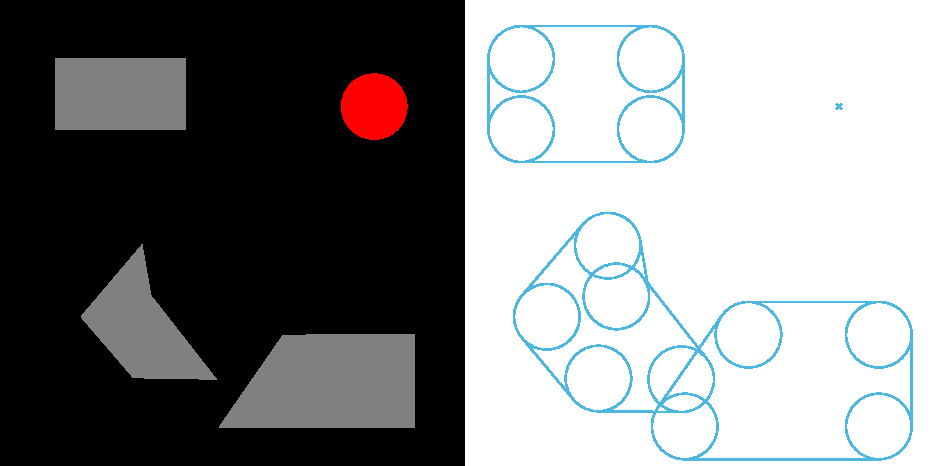
\includegraphics[width=0.9\textwidth]{doc/obrazky-figures/stage-logical.pdf}
%     \caption{Interní reprezentace herní plochy pro hledání kolizí s~překážkami. Vlevo je ukázka herní plochy tak, jak je prezentována uživateli, vpravo je převedena na interní reprezentaci.}
%     \label{fig:stage-logical}
% \end{figure}

% Algoritmus si interně vytváří model plochy, který se liší od způsobu, jakým je plocha prezentována na obrazovce. Zatímco překážky jsou vykreslovány jako mnohoúhelníky a~entity hráčů jako kruhy, interně jsou tyto tvary upraveny tak, aby se s~nimi lépe pracovalo. Všechny překážky jsou nejdříve upraveny tak, aby jejich vrcholy byly uspořádány proti směru hodinových ručiček. Stěny překážek jsou posunuty o~vzdálenost rovnu poloměru kruhu entity hráče, ve směru kolmém k této stěně. Rohy překážek ze změní v~kružnice se středem v~daném rohu a~poloměru stejném jako má entita hráče. Pak entita samotná se změní na pouhý bod v~rovině, který leží na stejných souřadnicích, jako střed kruhu entity hráče. Ukázka tohoto interního modelu je na obrázku~\ref{fig:stage-logical}.

% V~algoritmu je použito několik datových struktur. Jelikož algoritmus pracuje ve velké míře s~výpočty z~oblasti analytické a~výpočetní geometrie, mezi použité struktury patří \emph{bod}, \emph{vektor}, \emph{přímka}, \emph{úsečka}, \emph{kružnice} a~\emph{kruhový oblouk}. Krajní body \emph{úsečky} i~\emph{kruhového oblouku} jsou uspořádané, tedy jeden z~nich je vždy \emph{počáteční} a~druhý \emph{koncový}. \emph{Kruhový oblouk} může mít maximálně $180^\circ$ (avšak v~praxi nikdy nepřesáhne $90^\circ$). Další strukturou je \emph{úsek trajektorie}, který představuje buď \emph{úsečku}, nebo \emph{kruhový oblouk} (možná implementace v~jazyce \emph{C} by byla pomocí \emph{unie}). Také \emph{kolize s~překážkou} nebo \emph{hráč} jsou datové struktury. Jaké členy tyto struktury obsahují by mělo být zřejmé z~popisu algoritmu.

% Algoritmus dále pracuje s několika proměnnými:
% \begin{itemize}
%     \item $Traj$\,--\,seznam úseků trajektorie, představující celou trajektorii hráče,
%     \item $Tail$\,--\,zbývající úsek trajektorie po opuštění kolizní zóny s~překážkou (viz obrázek~\ref{fig:traj-tail}),
%     \item $MoveEnd$\,--\,přímka; hranice, kde končí hráčův pohyb,
%     \item $Flexible$\,--\,ohebnost posledního úseku trajektorie proměnné $Traj$. Může nabývat hodnot $CW$ (po směru hodinových ručiček\,--\,\emph{clockwise}), $CCW$ (proti směru hodinových ručiček\,--\,\emph{counterclockwise}) nebo $BOTH$ (ohebnost oběma směry), viz obázek~\ref{fig:flexible-both-cw},
%     \item $Coll$\,--\,informace o~poslední nalezené kolizi.
% \end{itemize}

% \begin{figure}[ht]
%     \centering
%     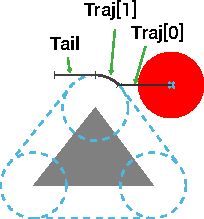
\includegraphics{doc/obrazky-figures/traj-tail.pdf}
%     \caption{Stav proměnných $Traj$ a~$Tail$ po vyhodnocení kolize s~rohem překážky. Při další iteraci hledání kolizí se z~$Tail$ stane $Traj[2]$.}
%     \label{fig:traj-tail}
% \end{figure}

% \begin{figure}[ht]
%     \centering
%     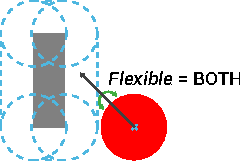
\includegraphics{doc/obrazky-figures/flexible-both.pdf}
%     \hspace{1cm}
%     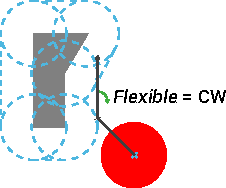
\includegraphics{doc/obrazky-figures/flexible-cw.pdf}
%     \caption{Hodnota proměnné $Flexible$ ve vztahu k~vybraným úsekům trajektorie. Vlevo je úsek ohebný oběma směry, vpravo pouze jedním směrem\,--\,po směru hodinových ručiček (\emph{clockwise}, \emph{CW}). Ohebnost úseku je v~obou případech také znázorněna zelenou šipkou.}
%     \label{fig:flexible-both-cw}
% \end{figure}

% Následuje samotný algoritmus popsaný sekvencí kroků. Jelikož tento algoritmus obsahuje poměrně velké množství kroků, byl rozdělen na několik částí. V~některých částech jsou některé kroky uzavřeny v~kulatých závorkách, což značí, že daný krok má být dále rozvinut v~jiné části algoritmu.

% \begin{enumerate}
%     \item Inicializuj:
%     \begin{itemize}
%         \item $Segment0$ jako úsek trajektorie představující požadovaný hráčův pohyb (úsečka vedoucí od aktuální pozice hráče ke koncovému bodu hráčova pohybu),
%         \item $Traj$ jako seznam obsahující pouze 1 položku\,--\,$Segment0$,
%         \item $Tail$ bez hodnoty,
%         \item $MoveEnd$ jako přímku kolmou na vektor hráčova pohybu, procházející bodem, kde končí hráčův pohyb,
%         \item $Flexible$ hodnotou $BOTH$ (ohebnost oběma směry).
%     \end{itemize}
%     \item \label{itm:trajectory-algo-1:begin-loop} Najdi kolizi $Coll$ posledního prvku seznamu $Traj$ s~překážkami.
%     \item Pokud nebyla nalezena žádná kolize, pak:
%     \begin{enumerate}
%         \item Pokud proměnná $Tail$ neobsahuje žádnou hodnotu, vrať $Traj$ jako výsledek; algoritmus končí.
%         \item Pokud proměnná $Tail$ obsahuje hodnotu (úsek trajektorie), připoj tuto hodnotu na konec seznamu $Traj$, nastav $Flexible$ na $BOTH$ a~vrať se na bod~\ref{itm:trajectory-algo-1:begin-loop}. Jinak pokračuj.
%     \end{enumerate}
%     \item \label{itm:trajectory-algo-1:call-process-coll} (Uprav hodnoty proměnných podle nalezené kolize $Coll$.)
%     \item Vrať se na bod~\ref{itm:trajectory-algo-1:begin-loop}.
% \end{enumerate}

% Výše je popsána základní část algoritmu, v~níž je provedena inicializace proměnných a~za ní následuje cyklus hledání kolizí. Je důležité si ujasnit, co je vnímáno jako \emph{kolize}: je to situace, kdy se kruh hráče překrývá s~překážkou. To znamená, že pokud se hráč pohybuje podél zdi nebo jeho pohyb končí nebo začíná těsně vedle zdi (přičemž během pohybu nedošlo k~překrytí s~překážkou), jedná se pouze o~\emph{dotek}, a~nikoliv o~\emph{kolizi}.

% Následuje část algoritmu vzniklá rozvinutím bodu~\ref{itm:trajectory-algo-1:call-process-coll} v~části algoritmu popsané výše:
% \begin{enumerate}
%     \item Nastav proměnnou $Tail$ do stavu bez hodnoty.
%     \item Nastav \emph{koncový bod} posledního prvku seznamu $Traj$ do bodu, kde nastala kolize.
%     \item Inicializuj nový úsek trajektorie $NewSegment$ podle kolize:
%     \begin{enumerate}
%         \item Pokud kolize nastala se stěnou překážky, pak $NewSegment$ bude \emph{úsečka}.
%         \item Pokud kolize nastala s~rohem překážky, pak $NewSegment$ bude \emph{kruhový oblouk} se středem stejným, jako je střed tohoto rohu.
%         \item \emph{Počáteční bod} bude v~obou případech v~bodě kolize. \emph{Koncový bod} zatím není znám.
%     \end{enumerate}
%     \item Urči přímku $Refl$, která je tečnou překážky v~bodě kolize.
%     \item Pokud je přímka $Refl$ kolmá na vektor hráčova pohybu, nastav koncový bod úseku $NewSegment$ do bodu kolize (bude to segment s~nulovou délkou), připoj jej na konec $Traj$ a~vrať $Traj$ jako výsledek; algoritmus končí (jedná se o~přímý náraz do překážky). Jinak pokračuj.
%     \item \label{itm:trajectory-algo-2:newsegment-flex} Urči ohebnost úseku $NewSegment$.
%     \item Pokud ohebnost úseku $NewSegment$ neodpovídá ohebnosti $Flexible$ (jsou různé a~zároveň $Flexible$ není $BOTH$), nastav koncový bod úseku $NewSegment$ do bodu kolize (bude to segment s~nulovou délkou), připoj jej na konec $Traj$ a~vrať $Traj$ jako výsledek; algoritmus končí (hráč se snaží projít příliš úzkým průchodem mezi překážkami). Jinak pokračuj.
%     \item Přepiš $Flexible$ hodnotou ohebnosti úseku $NewSegment$.
%     \item \label{itm:trajectory-algo-2:call-newsegment-endpoint} (Najdi \emph{koncový bod} úseku $NewSegment$.)
% \end{enumerate}

% Ohebnost úseku $NewSegment$ (bodě~\ref{itm:trajectory-algo-2:newsegment-flex}) se určí podle vztahu mezi vektorem pohybu hráče a~překážkou, jak je naznačeno na obrázku~\ref{fig:newsegment-wall-corner-flexible}. Pokud kolize nastala se stěnou překážky a~vektor pohybu hráče s~vektorem stěny svírají ostrý úhel (vektorem stěny je vektor z~\emph{počátečního} do \emph{koncového bodu} stěny), ohebnost je $CW$ (po směru hodinových ručiček). Pokud svírají tupý úhel, ohebnost je $CCW$ (proti směru hodinových ručiček). V~případě kolize s~rohem překážky 

% \begin{figure}
%     \centering
%     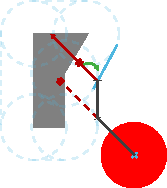
\includegraphics{doc/obrazky-figures/newsegment-wall-flexible.pdf}
%     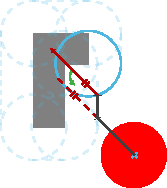
\includegraphics{doc/obrazky-figures/newsegment-corner-flexible.pdf}
%     \caption{Určení ohebnosti nového úseku trajektorie. Černá lomená čára ukazuje trajektorii pohybu hráče, červená šipka směr hráčova pohybu, zelená určenou ohebnost.}
%     \label{fig:newsegment-wall-corner-flexible}
% \end{figure}

% Další strukturou je úsek trajektorie, který představuje buď úsečku, nebo kruhový oblouk. Také na entitu hráče se nahlíží jako na datovou strukturu skládající se z~bodu, ve kterém se hráč nachází, a~vektoru hráčova pohybu.

% Níže je popsána procedura \textsc{Initialize}, která nastavuje výchozí hodnoty proměnných. Za zmínku stojí způsob, jakým je inicializována přímka $MoveEnd$ na řádku~\ref{alg:traj_old:line:init_MoveEnd}. Nezáleží totiž na její směrnici; přímka pouze nesmí být rovnoběžná s~vektorem pohybu hráče a~musí procházet bodem $MoveEndPt$. V~hlavním těle algoritmu bude počítán průsečík této přímky s~přímkou, po níž se pohybuje hráč, a~je nezbytně nutné, aby tento průsečík ležel právě v~bodě $MoveEndPt$.

% \begin{minipage}{\textwidth}
% \begin{algorithmic}[1]
%     \Procedure{Initialize}{$Traj$, $Tail$, $MoveEnd$, $Flexible$}
%         \State $Traj \gets \emptyset$
%         \State $Tail \gets NULL$
%         \State $MoveEndPt \gets Player.Position + Player.MovementVector$
%         \State $MoveEnd \gets$ \Call{Line}{$MoveEnd \perp Player.MovementVector \wedge MoveEndPt \in MoveEnd$} \label{alg:traj_old:line:init_MoveEnd}
%         \State $Flexible \gets BOTH$
%         \State $Segment0.Type \gets LINE\_SEGMENT$
%         \State $Segment0.PStart \gets Player.Position$
%         \State $Segment0.PEnd \gets MoveEndPt$
%         \State $Traj.$\Call{Push}{$Segment0$}
%     \EndProcedure
% \end{algorithmic}
% \end{minipage}

% \begin{minipage}{\textwidth}
% \begin{algorithmic}[1]
%     \Procedure{Main}{}
%         \State \Call{Initialize}{$Traj$, $Tail$, $MoveEnd$, $Flexible$}
%         \Loop
%             \State find the nearest $Collision$ of $Traj.Last$ with obstacles
%             \If{no $Collision$ was found}
%                 \If{$Tail = NULL$}
%                     \State \Return $Traj$
%                 \Else
%                     \State $Traj.$\Call{Push}{$Tail$}
%                     \State $Flexible \gets BOTH$
%                     \State $Tail \gets NULL$
%                 \EndIf
%             \Else
%             \EndIf
%         \EndLoop
%     \EndProcedure
% \end{algorithmic}
% \end{minipage}


% Pro kompilaci po částech (viz projekt.tex) nutno odkomentovat
%\end{document}
